% Chapter 1

\chapter{Το διαδίκτυο των αντικειμένων} % Main chapter title

\label{Chapter2} % For referencing the chapter elsewhere, use \ref{Chapter1} 

%\lhead{ΜΟΝΤΕΛΟΠΟΙΗΣΗ ΠΛΟΙΟΥ} % This is for the header on each page - perhaps a shortened title

%%%%%%%%%%%%%%%%%%%%%%%%%%%% The paper headers


%----------------------------------------------------------------------------------------

\section{Γενικά}
Το διαδίκτυο των αντικειμένων στην βιομηχανία αποτελεί μία νέα πρόταση για την διασύνδεση των βιομηχανικών μηχανη­μάτων και των αισθητήρων μεταξύ τους, μέσω του διαδικτύου, δί­νοντας έτσι στον χειριστή την δυνατότητα να χρησιμοποιήσει πληροφορίες που του παρέχονται από το κάθε αντικείμενο καθώς και να τις επεξεργαστεί ώστε να εξάγει χρήσιμα αποτελέσματα. 

Πριν την συγκεκριμένη τεχνολογία, στη βιομηχανία χρησιμοποιούνταν τεχνολογίες Blue-tooth και RFID, για τον έλεγχο και την παρακολούθηση βιομηχανικών εφαρμογών. Κάτι τέτοιο όμως περιοριζόταν σε μικρές αποστάσεις ελέγχου. Ο χειριστής θα έπρε­πε να βρίσκετε μέσα στο εύρος των Bluetooth ή μέσα στην περιο­χή που υπήρχαν οι συχνότητες των RFID. Την λύση σε αυτό το πρόβλημα έφερε η αυτοματοποίηση της βιομηχανίας μέσω του ΙοΤ. Χρησιμοποιώντας αυτή την τεχνολογία γίνεται εφικτός ο έλεγχος καθώς και η παρακολούθηση από οπουδήποτε στον κόσμο αρκεί να υπάρχει πρόσβαση στο διαδίκτυο [9]. Η εικόνα 2.1, που εμφανίζεται στο [9] δείχνει πως το ΙοΤ μπορεί να παρέχει διευκολύνσεις τόσο στην βιομηχανία όσο και σε διάφορους άλλους τομείς.


\begin{figure}[htbp]
	\centering
		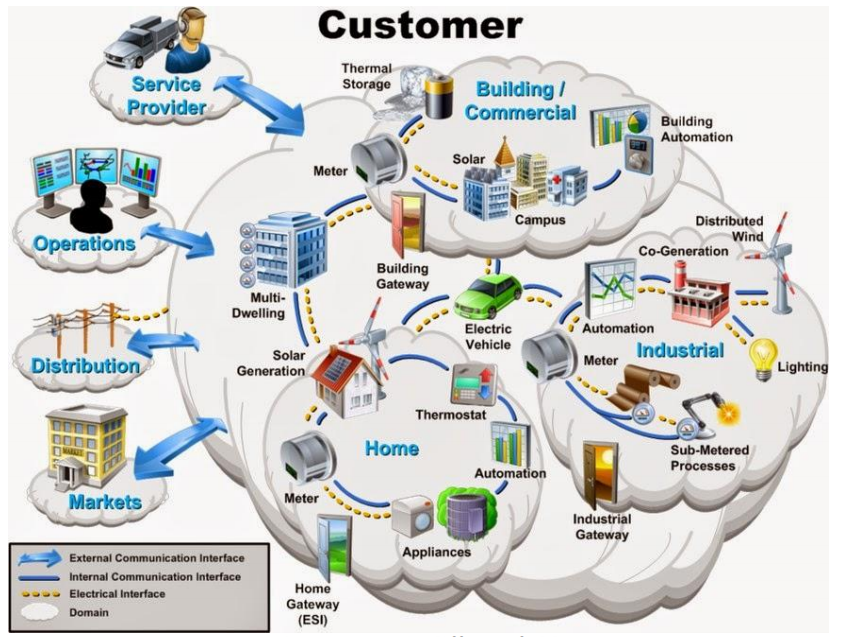
\includegraphics[height=8cm,width=12cm]{Figures/1.png}
	\caption{Το διαδίκτυο των αντικειμένων σε διάφορους τομείς \cite{Niranjan} }	
\end{figure}

%----------------------------------------------------------------------------------------
\section{Η κατάσταση μέχρι σήμερα}
Το διαδίκτυο των Αντικειμένων στη βιομηχανία βρίσκεται ακόμα σε πρώιμο στάδιο, παρόμοιο με αυτό που το διαδίκτυο βρισκόταν στα τέλη της δεκαετίας του 1990. Ενώ η εξέλιξη του διαδικτύου τις τελευταίες δύο δεκαετίες παρέχει κάποια σημαντικά διδάγματα, είναι αρκετά ασαφές το πως αυτή η γνώση μπορεί να αξιοποιηθεί στο Διαδίκτυο των Αντικειμένων στη βιομηχανία λόγω του μοναδικού πεδίου εφαρμογής του καθώς και λόγω των απαιτήσεων που υπάρχουν. Για παράδειγμα, οι αποκρίσεις σε πραγματικό χρόνο, είναι συχνά κρίσιμες στον κατασκευαστικό τομέα, στον τομέα της ενέργειας, της μεταφοράς καθώς και της υγείας. Ο πραγματικός χρόνος για το σημερινό Ίντερνετ συνήθως σημαίνει μερικά δευτερόλεπτα. Εν αντιθέσει, ο πραγματι­κός χρόνος σε ένα βιομηχανικό σύστημα είναι συχνά στην κλίμα­κα χιλιοστών του δευτερολέπτου Ο κανόνας του αντίχειρα (rule of thumb) υπαγορεύει ότι μία αλλαγή 10 φορές στην απόδοση απαι­τεί μία εντελώς διαφορετική προσέγγιση, για να μην αναφερθεί μια αλλαγή 100x  που θα επιφέρει στην βιομηχανία το Διαδίκτυο των Αντικειμένων [10].

Ένας άλλος σημαντικός παράγοντας πέρα από το χρόνο εί­ναι και η αξιοπιστία. Το ίντερνετ μέχρι στιγμής ακολουθεί μία προσέγγιση “καλύτερης προσπάθειας” (best-effort approach) η οποία παρέχει αποδεκτές επιδόσεις για τον άνθρωπο και για την αλληλεπίδραση του με το διαδίκτυο. Οι απροσδόκητες δυσλει­τουργίες σε έναν διακομιστή στην Google προκαλούν κάποιες κα­θυστερήσεις οι οποίες είναι αποδεκτές και δεν επηρεάζουν τόσο την αλληλεπίδραση του χρήστη με τις υπηρεσίες που του παρέχο­νται. Ωστόσο, η αποτυχία ενός ηλεκτρικού δικτύου, του συστήμα­τος ελέγχου της εναέριας κυκλοφορίας ή ενός αυτοματοποιημένου εργοστασίου για το ίδιο χρονικό διάστημα θα είχε πολύ πιο σοβα­ρές συνέπειες. 

Αυτοί οι παράγοντες της απόκρισης σε πραγματικό χρόνο και της αξιοπιστίας, που συνέβαλαν σε μία συντηρητική κουλτού­ρα μεταξύ των βιομηχανικών εταιρειών για την ενσωμάτωση των αλλαγών και των νέων τεχνολογιών, μαζί με το κόστος και την διάρκεια ζωής ενός τυπικού βιομηχανικού προϊόντος, είναι όλοι κρίσιμοι παράγοντες στη διαμόρφωση του τρόπου εξέλιξης του Διαδικτύου των Αντικειμένων στην Βιομηχανία.

Παρά τα εμπόδια αυτά, η υιοθέτηση του Διαδικτύου των Αντικειμένων στην βιομηχανία επιταχύνετε. Κατά τα τελευταία τρία χρόνια για παράδειγμα, ο αριθμός αισθητήρων που μεταφέρ­θηκαν αυξήθηκε περισσότερο από πέντε φορές. Πιο συγκεκρι­μένα, από 4,2 δισεκατομμύρια το 2012 αυξήθηκαν σε 23.6 δισεκα­τομμύρια το 2014 [11]. Μεγάλη προσοχή έχουν τραβήξει επίσης, οι προσπάθειες μεγάλων εταιρειών καθώς και κυβερνητικές πρω­τοβουλίες όπως το Industrie 4.0 [10].

Η Industry 4.0 είναι μία πολυετής στρατηγική πρωτοβουλία που πρόσφατα εισήγαγε η Γερμανική κυβέρνηση. Ο στόχος της πρωτοβουλίας αυτής είναι ο μετασχηματισμός της βιομηχανικής παραγωγής μέσω της ψηφιοποίησης και της εκμετάλλευσης των νέων δυνατοτήτων που προσφέρουν οι νέες τεχνολογίες. Η βιομη­χανική παραγωγή καθοδηγείται σήμερα από τον παγκόσμιο αντα­γωνισμό και την ανάγκη ταχείας προσαρμογής της παραγωγής στις συνεχώς μεταβαλλόμενες απαιτήσεις της αγοράς. Αυτές οι απαιτήσεις μπορούν να ικανοποιηθούν μόνο με ριζικές προόδους στην τρέχουσα τεχνολογία παραγωγής. Τα τεχνικά ζητήματα αυ­τών των απαιτήσεων αντιμετωπίζονται με την εφαρμογή των γε­νικών εννοιών των Cyber-Physical συστημάτων (CPS) και Διαδι­κτύου των Αντικειμένων στα συστήματα βιομηχανικής πα­ραγωγής [12].

Το Διαδίκτυο των Αντικειμένων στην βιομηχανία παρουσιάζεται σαν μία επανάσταση που υπόσχεται να αλλάξει ριζικά το πρόσωπο της βιομηχανίας. Στην πραγματικότητα, πρόκειται για μία εξέλιξη που έχει τις ρίζες της σε τεχνολογίες και λειτουργίες που έχουν αναπτυχθεί πριν από περισσότερα από 15 χρόνια. Η εμφάνιση του IIoT δημιούργησε τόσο ελπίδα όσο και σύγχυση σε φορείς που είναι υπεύθυνοι για την λειτουργία βιομηχανικών εγκαταστάσεων [13]. 

Ωστόσο, το Διαδίκτυο των Αντικειμένων στην βιομηχανία έχει να αντιμετωπίσει αρκετές προκλήσεις τόσο ερευνητικές όσο και τεχνολογικές. Οι πιο σημαντικές προκλήσεις που πρέπει να αντιμετωπιστούν σύμφωνα με την [14] είναι οι εξής:

\begin{enumerate}
	\item{\textbf{Τεχνολογική διαλειτουργικότητα}: Η διαλειτουργικότη­τα είναι σημαντικά πιο δύσκολη για το διαδίκτυο των αντικειμένων, καθώς δεν είναι μόνο η σύνδεση των ανθρώπων με τους ανθρώπους, αλλά η απρόσκοπτη αλληλεπίδραση μεταξύ συσκευών και ατόμων με συσκευές. Αυτές οι συσκευές μπορεί να διαφέρουν όσον αφορά τις τεχνολογικές τους δυνατότητες.}
	\item{\textbf{Σημασιολογική διαλειτουργικότητα}: Για να επιτευχθεί πλήρης διαλειτουργικότητα, είναι απαραίτητο οι συσκευές να ερμηνεύουν σωστά τις πληροφορίες κοινής χρήσης και να ενεργούν ανάλογα. Μία τέτοιου είδους διαλειτουργικότητα καλύπτεται από την σημασιολογι­κή πτυχή της διαλειτουργικότητας που συνήθως αναφέρεται σαν μοντέλο πληροφοριών (Information Model). Ως εκ τούτου, πρέπει να γίνουν βελτιώσεις όσον αφορά τις κατανεμημένες οντολογίες, τον σημα­σιολογικό ιστό (semantic web) καθώς και την ανακάλυ­ψη συσκευών μέσω σημασιολογίας. }
	\item{\textbf{Ασφάλεια και προστασία προσωπικών δεδομένων}: Η ακεραιότητα των δεδομένων, η μοναδική αναγνώριση καθώς και η κρυπτογράφηση θεωρούνται βασικές προκλήσεις για το Διαδίκτυο καθώς πολλά από τα δεδο­μένα που κοινοποιούνται περιέχουν προσωπικές πληροφορίες. Επιπλέον, τα δικαιώματα ιδιοκτησίας δεδο­μένων, τα νομικά ζητήματα και τα ζητήματα ευθύνης πρέπει να αντιμετωπιστούν αναλόγως. Τέλος, πρέπει να λαμβάνονται υπόψη οι ενεργειακά αποδοτικές τε­χνολογίες κρυπτογράφησης και προστασίας δεδομένων. }
	\item{\textbf{Έξυπνα αντικείμενα}: Πρέπει να αναπτυχθούν κυκλώμα­τα και συσκευές εξαιρετικά χαμηλής ισχύος ικανά να αντέχουν σε σκληρά περιβάλλοντα Επιπλέον, η παράλληλη επεξεργασία σε συστήματα πολλαπλών επεξεργαστών χαμηλής ισχύος, η προσαρμογή, η αυτόνομη συμπεριφορά με ταυτόχρονη εγγύηση της εμπιστοσύνης της ιδιωτικής ζωής και της ασφάλειας συγκαταλέγονται στις βασικές προκλήσεις όσον αφορά τις συσκευές του διαδικτύου. }
	\item{\textbf{Ανθεκτικότητα και αξιοπιστία}: Σε βιομηχανικά περιβάλλοντα ή σε περιπτώσεις έκτακτης ανάγκης, προσω­ρινές υπολειτουργίες του συστήματος δεν είναι αποδε­κτές. Ως εκ τούτου, τα ζητήματα ανθεκτικότητας και αξιοπιστίας στο διαδίκτυο πρέπει να διερευνηθούν από μια συνολική άποψη του συστήματος και επιπλέον πε­ριλαμβάνουν πτυχές όπως η διαθεσιμότητα, η ευρωστία και η ευελιξία της επικοινωνίας και του υλικού στις μεταβαλλόμενες περιβαλλοντικές συνθήκες, η αποφυγή ενιαίων σημείων αποτυχίας ή η ευρωστία δεδομένων επεξεργασίας σε αβέβαιες πληροφορίες. }
	
\end{enumerate}

Όταν αυτές οι προκλήσεις αντιμετωπιστούν, η διασύνδεση των βιομηχανικών συστημάτων παραγωγής με διάφορα άλλα συστήματα, συσκευές και καταναλωτές μέσω του διαδικτύου θα δημιουργήσει νέες δυνατότητες όπως αναφέρονται στο [15]: 

\begin{enumerate}
	\item{\textbf{Μαζική εξατομίκευση - Δημιουργία εξατομικευμένων προϊόντων με μικρούς χρόνους παράδοσης}: Πάντα υπήρχε ένας συμβιβασμός που έπρεπε να κάνει ένας κατασκευαστής μεταξύ εξατομίκευσης ενός προϊόντος και μαζικής παραγωγής του. Με την εφαρμογή του Δια­δικτύου των Αντικειμένων στην βιομηχανία ένα δι­κτυωμένο - έξυπνο εργοστάσιο καθιστά εφικτή την εξατομίκευση των προϊόντων σε κλίμακα μαζικής πα­ραγω-γής.}
	\item{\textbf{Συνεργασία ανθρώπου - μηχανής}: Η συνεργασία ανθρώπου - μηχανής μπορεί να διαχωριστεί σε φορητές διεπαφές ανθρώπου - μηχανής (mobile Hu­man-Machine Interfaces, HMI) και συνεργατικά συστήματα ανθρώπου - μηχανής (Human-Machine Collaborative Systems, HMCS). Οι HMI τεχνολογίες, για παράδειγμα κινητά τηλέφωνα, ταμπλέτες, ηλεκτρονικά που φοριούνται (wearables) σε συνδυασμό με πρόσβαση στο διαδίκτυο θα αλλάξουν ριζικά τον τρόπο με τον οποίο οι χειρι­στές των μηχανών και οι μηχανικοί θα παρακολουθούν και θα χειρίζονται την παραγωγή. Η φυσική παρουσία του προσωπικού στο χώρο διαχείρισης δεν θα είναι απαραίτητη, γεγονός που αυξάνει την ασφάλεια και οι ικανότητες του χειριστή διευρύνονται με την χρήση νέων τεχνολογιών όπως η εικονική πραγματικότητα για την καλύτερη παρακολούθηση της παραγωγής και τον εντοπισμό των προβλημάτων. Οι HMCS τεχνολογί­ες στοχεύουν στην κατασκευή ευέλικτων ρομποτικών συστημάτων για κατασκευαστές μικρής κλίμακας οι οποίοι τροποποιούν συχνά τις γραμμές παραγωγής τους. Η δυνατότητα ανάλυσης αλυσίδας ενεργειών (Action Sequence analysis) θα δίνει τη δυνατότητα στα ρομποτικά συστήματα αυτά να “μαθαίνουν” δυναμικά νέες εργασίες όπως η συναρμολόγηση κάποιου νέου προϊόντος με επαναληπτικές μεθόδους αντί για προ­γραμματισμό, πράγμα που μπορεί εύκολα να γίνει από ένα εργαζόμενο χωρίς αυτός να έχει ιδιαίτερες γνώσεις προγραμματισμού. }
	\item{\textbf{Ενοποίηση της παγκόσμιας αλυσίδας εφοδιασμού}: Η παγκοσμιοποίηση της αγοράς και των αλυσίδων εφοδιασμού, παρόλο που είναι εξαιρετικά κερδοφόρα για τον κατασκευαστή, δημιουργεί ορισμένα προβλήματα. Οι κατασκευαστές οφείλουν να λαμβάνουν υπ’ όψη τους πολλούς παράγοντες όπως οι τρέχουσες τιμές, διαθεσιμότητες, χρόνοι παράδοσης, ποιοτικές προδια­γραφές και αποθέματα πρώτων υλών, εργαλείων και μηχανών. Στα πλαίσια του Διαδικτύου των Αντικει­μένων στην βιομηχανία αναπτύσσονται εργαλεία τα οποία παρέχουν ενοποιημένη πρόσβαση σε πραγματικό χρόνο στις πληροφορίες αυτές. Κάτι τέτοιο ενισχύει την παραγωγικότητα, την ασφάλεια στο χώρο εργασίας και την ποιότητα της παραγωγής.}
\end{enumerate}

Η εφαρμογή της τεχνολογίας του Διαδικτύου των Αντικειμένων σε τομείς της βιομηχανίας αναμένεται να έχει έντονο αντίκτυπο σε όλη την διαδικασία της παραγωγής ώστε τελικά να οδηγήσει στην επονομαζόμενη τέταρτη βιομηχανική επανάσταση. Η εικόνα 2.2 δείχνει τις φάσεις που πέρασε η βιομηχανική επανάσταση.

\begin{figure}[htbp]
	\centering
		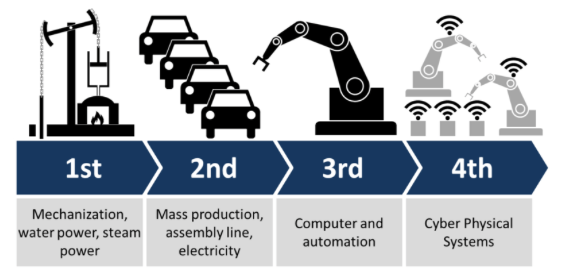
\includegraphics[height=7.5cm,width=15cm]{Figures/2.png}
	\caption{Οι φάσεις των βιομηχανικών επαναστάσεων \cite{Marr} }	
\end{figure}

Οι πιο αισιόδοξες προβλέψεις κάνουν λόγο για παραγωγή επιπρόσθετης αξίας παγκοσμίως από την εφαρμογή τους Διαδι­κτύου των Αντικειμένων στην βιομηχανίας της τάξης των 15 τρισεκατομμυρίων δολαρίων μέχρι το 2030 [16].  
%----------------------------------------------------------------------------------------
\section{Πρότυπα και πρωτόκολλα ΙοΤ}
Στο όραμα του Διαδικτύου των Αντικειμένων, το διαδίκτυο εξαπλώνεται πέρα από τον πυρήνα του. Αυτή η τεράστια ανάπτυ­ξη φέρνει τόσο συναρπαστικές δυνατότητες όσο και προκλήσεις στο Διαδίκτυο, όπως το πως θα ενσωματωθούν απρόσκοπτα οι διάφορες συσκευές και οι σένσορες στον παγκόσμιο ιστό. Ένας τρόπος για την ομαλή ενοποίηση του κυβερνο-κόσμου  και του φυσικού κόσμου είναι η επαναχρησιμοποίηση των υφιστάμενων τεχνολογιών και προτύπων στον παγκόσμιο ιστό, όσο το δυνατόν περισσότερο. Αυτή την τάση έρευνας την αντιμετωπίζει το Διαδί­κτυο των Αντικειμένων ως το Διαδίκτυο των πραγμάτων (Web of Things, WoT). Στο WoT, οι συσκευές δεν έχουν απλά μία ΙΡ ώστε να είναι συνδεδεμένες στο διαδίκτυο, αλλά έχουν την δυνατότητα να μιλούν και την ίδια γλώσσα και έτσι είναι σε θέση να επικοινω­νούν και να αλληλεπιδρούν ελεύθερα στον Παγκόσμιο Ιστό. Προ­κειμένου να υλοποιηθεί αυτό το όραμα, πρέπει να διεξαχθεί εκ νέου σχεδιασμός και βελτιώσεις στην κωδικοποίηση ωφέλιμου φορτίου και στα πρωτόκολλα εφαρμογής, ώστε να ικανοποιηθούν οι ειδικές απαιτήσεις των εφαρμογών μηχανής προς μηχανή (Machine to Machine, M2M) σε περιορισμένα περιβάλλοντα του διαδικτύου των αντικειμένων [17].

	Ένας τρόπος να εκπληρωθούν τα παραπάνω ζητούμενα είναι η ευρεία τοποθέτηση κοινής αρχιτεκτονικής, τόσο σε επίπεδο δικτύου, το οποίο επιτυγχάνεται με τα 6LoWPAN πρότυπα [19], όσο και σε επίπεδο εφαρμογών μέσω του WoT [20] που αναφέρθηκε παραπάνω. Μία τέτοια προσέγγιση επιτυγχάνει την χαλαρή ζεύξη (loose coupling) μεταξύ των τμημάτων που αποτελούν μια κατα­νεμημένη εφαρμογή, ιδιότητα - κλειδί για την επίτευξη της ζητού­μενης διαλειτουργικότητας [18]. 
	
\subsection{Η αρχιτεκτονική REST}
Η αρχιτεκτονική αρχή που βρίσκεται στην καρδιά του διαδικτύου, δηλαδή η Representatio-nal State Transfer (REST) όπως ορίστηκε από τον Roy Fielding [31], μοιράζεται έναν παρόμοιο στόχο με τις περισσότερες γνωστές τεχνικές ενοποίησης όπως οι υπηρεσίες WS-*  Web  services  (SOAP,  WSDL,  κτλ), ο οποίος εί­ναι η αύξηση της διαλειτουργικότητας για μια χαλαρότερη ζεύξη μεταξύ τμημάτων των κατανεμημένων εφαρμογών. Ωστόσο, ο στόχος του REST είναι να το επιτύχει αυτό με έναν πιο ελαφρύ και απλούστερο τρόπο και εστιάζει σε πόρους και όχι σε λειτουργίες, όπως συμβαίνει με τις υπηρεσίες WS-* Web. Συγκεκριμένα, το REST χρησιμοποιεί το Διαδίκτυο ως μια πλατφόρμα εφαρμογών και εκμεταλλεύεται πλήρως όλες τις λειτουργίες που είναι εγγε­νείς στο HTTP πρωτόκολλο, όπως ο έλεγχος ταυτότητας, η εξου­σιοδότηση, η κρυπτογράφηση, η συμπίεση και η προσωρινή απο­θήκευση. Με αυτόν τον τρόπο το REST “φέρνει” υπηρεσίες μέσα στον πρόγραμμα περιήγησης. Οι πόροι μπορούν να συνδεθούν και να ανατεθούν σε σελιδοδείκτες και τα αποτελέσματα να είναι ορατά με οποιοδήποτε πρόγραμμα περιήγησης του ιστού χωρίς να χρειάζεται να παράγουν πολύπλοκο πηγαίο κώδικα από αρχεία WSDL για να μπορούν να αλληλεπιδρούν με μία υπηρεσία [18]. 
	
	Για να το πετύχει αυτό η REST αρχιτεκτονική απαρτίζεται από δύο βασικούς κανόνες: 
	
\begin{itemize}
	\item{Το μοντέλο εφαρμογής μετασχηματίζεται και αντί να έχει την λειτουργικότητα σαν κύριο άξονα έχει τα δεδο­μένα. Αυτό σημαίνει ότι κάθε τι που προσφέρει υπηρε­σίες γίνεται πλέον ένας πόρος (resource), για παράδειγμα ένας αισθητήρας θερμότητας είναι ένας πόρος, που μπορεί να αναγνωριστεί μέσω ενός συγκεκριμένου URI.}
	\item{Οι τέσσερις κύριες λειτουργίες που παρέχονται από το πρωτόκολλο HTTP (PUT, POST, GET, DELETE) είναι οι μόνες διαθέσιμες λειτουργίες που μπορεί να έχει ένας πόρος. Έτσι ορίζεται μια ομοιόμορφη διεπαφή με γνωστή και κοινή σημασιολογία. }
\end{itemize}

 Αυτά τα πλεονεκτήματα εξηγούν κυρίως γιατί οι υπηρεσίες που προσφέρει η REST αρχιτεκτονική αποτελούν την τεχνολογική βάση για ένα αυξανόμενο αριθμό υπηρεσιών Web 2.0 όπως αυτές που προσφέρονται από το Flickr, το Twitter, το Google και το Amazon. Παραδοσιακά, η REST αρχιτεκτονική έχει χρησιμοποιη­θεί για την ενσωμάτωση διάφορων υπηρεσιών που παρέχονται σε ιστοσελίδες. Ωστόσο, επειδή η αρχιτεκτονική αυτή είναι αρκετά ελαφριά γίνεται άμεσα υποψήφια για ενσωματωμένες συσκευές με περιορισμένους πόρους ώστε να προσφέρουν υπηρεσίες στον παγκόσμιο ιστό. Εφόσον, τέτοιες συσκευές προσφέρουν συνήθως απλές και ατομικές λειτουργίες η μοντελοποίησή τους χρησιμοποιώντας το REST είναι συχνά απλή [18]. 

	Έχει σημασία να επισημανθεί πως το REST δεν περιγράφει κάποιο συγκεκριμένο πρωτόκολλο αλλά έχει μόνο ένα στυλ σχεδιασμού πρωτοκόλλων επικοινωνίας.

\subsection{Τα πρωτόκολλα HTTP - CoAP}
Επί του παρόντος, η πρόσβαση στο Διαδίκτυο απαιτεί πρωτόκολλα εφαρμογών μέσω TCP / IP  ή UDP / IP. Ένα τέτοιο πρωτόκολλο εφαρμογής αποτελεί το Hyper Text Transfer Protocol (HTTP), το οποίο έχει τυποποιηθεί στο ΙΕTF, και έχει εφαρμοστεί για την επικοινωνία στο διαδίκτυο. Ωστόσο, όταν εφαρμόζεται αυτό το πρωτόκολλο στην επικοινωνία μεταξύ συσκευών στο ΙοΤ, κατά την οποία μεταφέρεται ένας τεράστιος αριθμός μικροσκοπι­κών μπλοκ δεδομένων, το overhead που προστίθεται σε συνδυα­σμό με τις χαμηλές επιδόσεις αποτελούν ένα σημαντικό πρόβλη­μα. Επιπλέον, η διεύθυνση ΙΡ εξαρτάται από την φυσική τοποθε­σία της συσκευής, γεγονός που δημιουργεί το πρόβλημα της πολυπλοκότητας του ελέγχου δικτύου. 

	 Επιπλέον ένα μέρος της διαδρομής του δικτύου που θα ακολουθούν τα δεδομένα θα είναι μέσα σε δίκτυα χαμηλής ισχύος και με υψηλό ποσοστό απώλειας δεδομένων (Low power and Lossy Networks, LLN) [21]. Έτσι λοιπόν ένα κατάλληλο για την M2M επικοινωνία πρωτόκολλο πρέπει να μεγιστοποιεί την εξοικονόμηση ενέργειας, να είναι αποδοτικό όταν χρησιμοποιείται σε LLN’s και να είναι σχετικά ελαφρύ ώστε να εκτελείται σε μικρών δυνατοτή­των (μνήμης και επεξεργαστικής ισχύος) ενσωματωμένα συστή­ματα. Επιπρόσθετα το HTTP δε διαθέτει κάποιο μηχανισμό για αποστολή multi cast και εντοπισμού resources.

	Τα προβλήματα αυτά έρχεται να λύσει το πρωτόκολλο Constrained Application Protocol (CoAP). Το CoAP είναι ένα πρωτόκολλο σύγχρονης αίτησης / απόκρισης επιπέδου εφαρμογής που σχεδιάστηκε από την Internet Engineering Task Force (IETF) για να στοχεύσει σε συσκευές περιορισμένων πόρων. Σχεδιάστη­κε χρησιμοποιώντας ένα υποσύνολο των μεθόδων του πρωτοκόλ­λου HTTP που το καθιστούν διαλειτουργικό με το HTTP [23]. 

	Το  CoAP λειτουργεί πάνω από UDP έτσι ώστε να είναι όλη η υλοποίησή του ελαφριά. Χρησιμοποιεί τις εντολές του ΗΤΤΡ, GET, POST, PUT και DELETE για την παροχή αλληλεπιδράσεων προσανατολισμένων σε πόρους σε μια αρχιτεκτονική πελάτη - διακομιστή (client - server). Το CoAP είναι ένα πρωτόκολλο  αίτησης / απόκρισης που χρησιμοποιεί τόσο σύγχρονες όσο και ασύγχρονες απαντήσεις. Ο λόγος για το σχεδιασμό ενός πρωτοκόλλου επι­πέδου εφαρμογής που βασίζεται σε UDP για την διαχείριση των πόρων είναι η κατάργηση του overhead που προσθέτει το TCP και η μείωση των απαιτήσεων σχετικά με το εύρος ζώνης [24]. Χρησι­μοποιώντας το αναξιόπιστο UDP, το CoAP υλοποίησε τους δικούς του μηχανισμούς για την επίτευξη αξιοπιστίας. Δύο bit στην κε­φαλίδα κάθε πακέτου αναφέρουν τον τύπο του μηνύματος και το απαιτούμενο επίπεδο ποιότητας υπηρεσίας (QoS).  Υπάρχουν τέσ­σερις τύποι μηνυμάτων: 
	
\begin{enumerate}
	\item{\textbf{Επιβεβαιώσιμο}: Ένα μήνυμα αίτησης που απαιτεί επιβεβαίωση (ACK). Η απόκριση μπορεί να αποσταλεί είτε συγχρόνως (εντός του ACK) είτε εάν χρειάζεται περισσότερος υπολογιστικός χρόνος, μπορεί να σταλεί ασύγχρονα με ένα ξεχωριστό μήνυμα.}
	\item{\textbf{Μη επιβεβαιώσιμο}: Ένα μήνυμα που δεν απαιτεί επιβεβαίωση.}
	\item{\textbf{Αναγνώρισης}: Επιβεβαιώνει τη λήψη ενός επιβεβαίωσιμου μηνύματος.}
	\item{\textbf{Επαναφοράς (Reset)}: Επιβεβαιώνει την λήψη ενός μηνύματος που δεν είναι δυνατή η επεξεργασία του.}
\end{enumerate}

Υπάρχει επίσης ένας απλός μηχανισμός μετάδοσης Stop - and - Wait για επιβεβαιωμένα μηνύματα και ένα πεδίο κεφαλίδας 16 bit σε κάθε πακέτο CoAP ονομάζεται message ID, το οποίο εί­ναι μοναδικό και χρησιμοποιείται για την ανίχνευση διπλότυπων.  

	Παρόλο που το CoAP δημιουργήθηκε για τις επικοινωνίες ΙοΤ και Μ2Μ, δεν περιλαμβάνει ενσωματωμένα χαρακτηριστικά ασφαλείας. Το πρωτόκολλο που προτείνεται για διασφάλιση των συναλλαγών μέσω του CoAP είναι το Datagram Transport Layer Security (DTLS) [25].

	Η εικόνα 2.3 αναπαριστά την αρχιτεκτονική του πρωτοκόλλου CoAP: 
	
	
\begin{figure}[htbp]
	\centering
		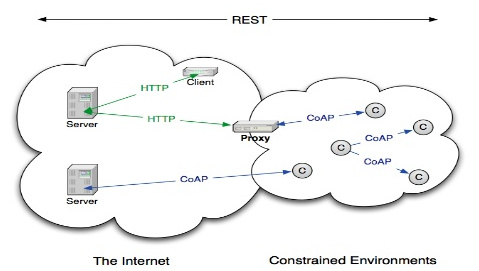
\includegraphics[height=8cm,width=12cm]{Figures/3.jpg}
	\caption{Η αρχιτεκτονική CoAP \cite{Coap} }	
\end{figure}

\subsection{Το πρωτόκολλο MQTT}
Το Message Queue Telemetry Transport (MQTT) πρωτόκολλο κυκλοφόρησε από την ΙΒΜ και στοχεύει σε ελαφρές επικοινωνίες μεταξύ συσκευών (Μ2Μ). Πρόκειται για ένα ασύγχρονο πρωτόκολλο δημοσίευσης / εγγραφής (publish / subscribe) που εκτελείται στην κορυφή του TCP.  Τα πρωτόκολλα δημοσίευσης / εγγραφής πληρούν καλύτερα τις απαιτήσεις του IoT από τα πρωτόκολλα αιτήματος / απόκρισης (request /response), δεδομένου ότι οι clients δεν χρειάζεται να ζητούν ενημερώσεις και έτσι το εύρος ζώνης του δικτύου μειώνεται και η ανάγκη χρήσης υπολογιστικών πόρων μειώνεται. 

Στο MQTT υπάρχει ένας broker (διακομιστής) που περιέχει ζητήματα. Κάθε πελάτης (client) μπορεί να είναι ένας εκδότης (publisher) που στέλνει πληροφορίες στον broker σχετικά με ένα συγκεκριμένο ζήτημα ή / και έναν συνδρομητή (subscriber) που λαμβάνει αυτόματα μηνύματα κάθε φορά που υφίσταται μία αλλαγή σε ένα ζήτημα στο οποίο έχει εγγραφεί. Το συγκεκριμένο πρωτόκολλο έχει σχεδιαστεί για να χρησιμοποιεί το εύρος ζώνης και τη χρήση μπαταρίας με φειδώ γι’ αυτό για παράδειγμα αυτή τη στιγμή χρησιμοποιείται από το Facebook Messenger [26]. 

Το ΜQTT εξασφαλίζει αξιοπιστία παρέχοντας την επιλογή τριών επιπέδων QoS: 
\begin{enumerate}
	\item{\textbf{Fire and forget}: Ένα μήνυμα αποστέλλεται μία φορά και δεν απαιτείται επιβεβαίωση.}
	\item{\textbf{Delivered at least one}: Ένα μήνυμα αποστέλλεται τουλάχιστον μία φορά και απαιτείται επιβεβαίωση.}
	\item{\textbf{Delivered exactly one}: Ένας μηχανισμός χειραψίας τεσσάρων κατευθύνσεων χρησιμοποιείται για να εξασφαλίσει ότι το μήνυμα παραδίδεται ακριβώς μία φορά. }
\end{enumerate}

Aξίζει να σημειωθεί ότι παρόλο που το MQTT τρέχει πάνω από το TCP, έχει σχεδιαστεί ώστε να προσθέτει χαμηλό overhead σε σύγκριση με άλλες εφαρμογές που βασίζονται στο TCP [27]. Η εικόνα 2.4 δείχνει την αρχιτεκτονική του MQTT  πρωτοκόλλου.


\begin{figure}[htbp]
	\centering
		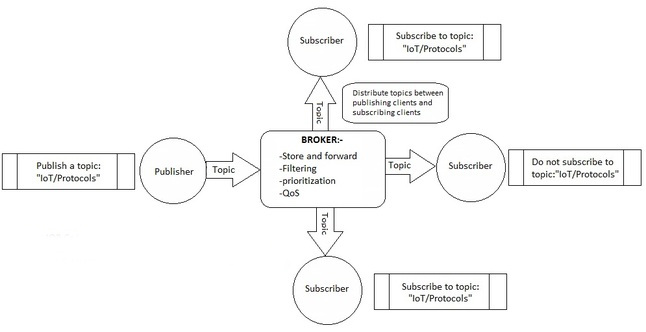
\includegraphics[height=8cm,width=15cm]{Figures/4.jpg}
	\caption{Η αρχιτεκτονική MQTT \cite{Gupta} }	
\end{figure}

Ενδεικτικά, άλλα διαδεδομένα πρωτόκολλα είναι τα XMPP, DDS, SOAP και WebSocket.

